\documentclass[a4paper,12pt,twoside]{report} 
\usepackage{times}
\usepackage{amsmath}
\usepackage[top=30mm, bottom=15mm, left=20mm, right=20mm]{geometry}
\usepackage{multirow}
\usepackage{hhline}
\usepackage{epigraph}
\usepackage{fancyhdr}
\usepackage{ragged2e}

\usepackage{enumitem,wrapfig}
\usepackage{graphicx}

\usepackage{pdflscape}

\usepackage{amssymb}

%% Escrevendo em português
\usepackage[english,brazil]{babel}
\usepackage[utf8]{inputenc}

\usepackage[nodayofweek]{datetime}

\usepackage[titletoc]{appendix}

\usepackage[nottoc,notlot,notlof,numbib]{tocbibind}

\usepackage{color}

\definecolor{pblue}{rgb}{0.13,0.13,1}
\definecolor{pgreen}{rgb}{0,0.5,0}
\definecolor{pred}{rgb}{0.9,0,0}
\definecolor{pgrey}{rgb}{0.46,0.45,0.48}

\usepackage{listings}
\lstset{language=Matlab,
  showspaces=false,
  showtabs=false,
  breaklines=true,
  showstringspaces=false,
  breakatwhitespace=true,
  commentstyle=\color{pgreen},
  keywordstyle=\color{pblue},
  stringstyle=\color{pred},
  %basicstyle=\ttfamily,
  basicstyle=\footnotesize\tt,
  moredelim=[il][\textcolor{pgrey}]{$$},
  moredelim=[is][\textcolor{pgrey}]{\%\%}{\%\%},
  tabsize=2,
  literate={\ \ }{{\ }}1
}

\linespread{1.1}

\fancypagestyle{IHA-fancy-style}{%
  \fancyhf{}% Clear header and footer
  \fancyhead[LE,LO]{{\scriptsize MGPU: Mapa Geográfico de Problemas Urbanos}}
  \fancyhead[RO,RE]{{\scriptsize Engenharia de Usabilidade para Sistemas Web}}
  \fancyfoot[C]{\thepage}
  \renewcommand{\headrulewidth}{0pt}% Line at the header invisible
  \renewcommand{\footrulewidth}{0pt}% Line at the footer visible
}

% Redefine the plain page style
\fancypagestyle{plain}{%
  \fancyhf{}%
  \fancyhead[LE,LO]{{\scriptsize MGPU: Mapa Geográfico de Problemas Urbanos}}
  \fancyhead[RO,RE]{{\scriptsize Engenharia de Usabilidade para Sistemas Web}}
  \fancyfoot[C]{\thepage}
  \renewcommand{\headrulewidth}{0pt}% Line at the header invisible
  \renewcommand{\footrulewidth}{0pt}% Line at the footer visible
}

%% Início documento
\begin {document}
\thispagestyle{empty}

% Capa
\begin{titlepage}
  \centering
  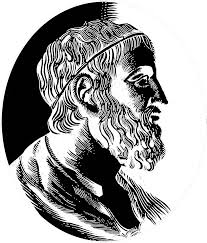
\includegraphics[width=0.15\textwidth]{ime_logo}\par\vspace{1cm}
   {\scshape\LARGE Instituto de Matemática e Estatística \\ Universidade de São Paulo \par}
  \vspace{1cm}
  {\scshape\large  Curso de verão \par}
  {\scshape\normalsize  Engenharia de Usabilidade para Sistemas Web\par}
  \vspace{1.5cm}
  {\LARGE\bfseries MGPU: Mapa Geográfico de Problemas Urbanos\par}
  
  \vspace{2cm}
  {\Large\itshape Grupo: \par}
  {\Large\itshape António Augusto Tavares Martins Miranda\par}
  {\Large\itshape Thiago de Jesus Inocêncio\par}
  {\Large\itshape Wagner Santos C. de Jesus\par}
  \vfill
  Professor\par
  Hamilton Fernandes de Moraes Junior

  \vfill

  % Bottom of the page
  {\large São Paulo, Janeiro de 2017}
\end{titlepage}

\newpage

\pagestyle{IHA-fancy-style}

\newpage

%% Sumário
\tableofcontents

\newpage

\chapter{Introdução}

Ao longo do curso de Engenharia de Usabilidade em Sistemas Web, ministrado pelo prof. Hamilton Fernandes de Moraes Júnior, foram abordados os principais conceitos da engenharia de usabilidade, design de interação, experiência do usuário, foi estudado problemas típicos de sites web, prototipação, avaliação de usabilidade e por fim conceitos de acessibilidade em web.
\\~\\
Tendo em conta que esses conceitos podem ser aplicados universalmente para o desenvolvimento de qualquer software que interaja com humanos, e devido a crescente relevância das aplicações \textit{mobile}, e visando também a avaliação da turma, foi-nos proposto o desenvolvimento de um aplicativo \textit{mobile} usando os conceitos e técnicas aprendidos ao longo do curso. Disso surgiu o MGPU (Mapa Geográfico de Problemas Urbanos), trata-se de um aplicativo colaborativo que permite fazer o mapeamento de problemas urbanos de uma cidade ou bairro. Fazendo o uso da sua interface simples e minimalista, sem sacrifício da experiência, o usuário poderá facilmente visualizar e reportar os problemas urbanos aos órgãos responsáveis.

\section{Objetivos}

O MGPU foi criado como um meio de experienciar em primeira mão as dificuldades e os desafios resultantes da aplicação dos conceitos e técnicas de engenharia de usabilidade, permitindo também a realização da importância da aplicação dos mesmos no processo de desenvolvimento de softwares interativos.  

\section{Publico alvo}

O público alvo do MGPU é qualquer pessoa com um \textit{smartphone} que se preocupa com os problemas urbanos e está disposta a contribuir na resolução dos mesmos.

\clearpage

\section{Justificativa}

Devido a sua relevância social, o aplicativo MGPU foi o esolhido para ser desenvolvido. Ele tem o potencial de revolucionar a forma como as grandes cidades lidam e resolvem os seus problemas urbanos. Com o mapeamento colaborativo de problemas urbanos, os órgãos responsáveis poderão facilmente localizar-los, permitindo uma diminuição no tempo de resposta e resolução desses problemas, e aumento da qualidade de vida nos centros urbanos.

\chapter{Personas e cenários}
Personas são as representações fictícias do seu público do produto. Elas permitem aos membros da equipe conhecer e entender melhor os consumidores do produto, orienta a tomada de decisões para o consumidor e ajudam a identificar lacunas e novas oportunidades no produto.\cite{R0}
\\~\\
O Cenário descreve um contexto na qual as personas estão inseridas e ajuda a visualizar os conceitos de \textit{design}.\cite{R0}

\section{1º Par persona/cenário}
\subsection{Persona}
\begin{itemize}
\item \textbf{Nome:} Carla Patrícia Cavalcanti.
\item \textbf{Idade:} 40.
\item \textbf{Sexo:} Feminino.
\item \textbf{Nível de escolaridade:} Ensino médio completo.
\item \textbf{Profissão:} Recepcionista.
\item \textbf{Localização:} Avenida Marechal Fiúza de Castro, São Paulo.
\item \textbf{Perfil:} Carla tem 40 anos, casada e mãe de dois filhos. Ela é muito devota aos filhos e na medida do possível tenta dar tudo do melhor para eles. Trabalha como recepcionista num escritório na Avenida Paulista e usa como principal meio de transporte o metrô. Carla está sempre bem informada sobre as notícias no Brasil e no mundo. Aderiu facilmente ao mundo das novas tecnologias e é fã de redes sociais como \textit{facebook} e \textit{twitter}. Sempre que o tema de uma atividade social é qualidade de vida no meio urbano ela tenta participar.
\item \textbf{Estilo de vida:} Após o trabalho ela passa o tempo cuidando da casa, do marido, dos filhos e das suas plantas. Sempre que possível, a Carla adora levar os filhos para brincar na praça e aproveitar para colocar a conversa em dia com as amigas. Aos fins de semana ela incentiva o marido a fazer alguma atividade física acompanhando-o nos passeios de bicicleta pela cidade.
\item \textbf{Objetivos:} Garantir um futuro melhor para os filhos e se possível arranjar fundos e meios para melhorar a qualidade de vida e segurança no seu bairro.
\end{itemize}
\subsection{Cenário}
Carla, juntamente com os filhos, a caminho do local na praça onde costuma se encontrar com as amigas, ela se depara com uma árvore caída no chão e obstruindo parte da estrada. Por ser uma pessoa bem informada e preocupada com a qualidade de vida zonas urbanas, ela sabia da existência de um aplicativo para reportar problemas urbanos. Como a situação envolvendo a árvore era de risco ela decidiu baixar o aplicativo e submeter uma ocorrência anônima da queda da árvore e com fotos para comprovar a autenticidade da ocorrência.

\section{2º Par persona/cenário}
\subsection{Persona}
\begin{itemize}
\item \textbf{Nome:} Marcos Almeida.
\item \textbf{Idade:} 20.
\item \textbf{Sexo:} Masculino.
\item \textbf{Nível de escolaridade:} Nível superior em andamento.
\item \textbf{Profissão:} Estudante.
\item \textbf{Localização:} Avenida São Remo, São Paulo.
\item \textbf{Perfil:} Marcos faz bacharelato em letras, é uma pessoa muito atenciosa e compreensiva, adora viajar e conhecer pessoas novas. Na faculdade ele faz parte da comissão de recepção dos caloiros do curso de letras. Os principais meios de locomoção do Marcos são ônibus, metrô e bicicleta. Marcos é vegetariano e muito apreciador da cultura e música nacional. Marcos também é fascinado pela política e está sempre bem informado sobre o assunto.   
\item \textbf{Estilo de vida:} Quando não se encontra na faculdade, Marcos toca piano numa pequena orquestra de amigos, passa tempo com a namorada e joga futsal. Nos finais de semana, Marcos nunca perde uma ida ao bar para beber e discutir políticas para melhorar a cidade de São Paulo. 
\item \textbf{Objetivos:} Após a faculdade ele quer fazer um mestrado, e talvez de seguida entrar na política e contribuir com desenvolvimento e melhoria da sua cidade. Ele também gostaria muito viajar para a Europa.
\end{itemize}
\subsection{Cenário}
Quando ia para a faculdade de bicicleta, Marcos reparou que o semáforo perto da portaria da universidade estava funcionando incorretamente, o que é inaceitável e põe em risco a vida de motoristas e pedestres. Após se encontrar numa localização segura e favorável, Marcos usa o aplicativo MGPU para filmar o funcionamento indevido do semáforo e abrir uma ocorrência de um problema urbano na sua localização.

\clearpage
 
\section{3º Par persona/cenário}
\subsection{Persona}
\begin{itemize}
\item \textbf{Nome:} Luís Carlos.
\item \textbf{Idade:} 57.
\item \textbf{Sexo:} Masculino.
\item \textbf{Nível de escolaridade:} Doutorado em Psicologia.
\item \textbf{Profissão:} Professor Universitário.
\item \textbf{Localização:} Rua Doutor Artur Guimarães, São Paulo.
\item \textbf{Perfil:} Doutorado em Psicologia, Luís é professor universitário e coordenador do curso de psicologia. Passa maior parte do tempo fazendo pesquisas, é separado e tem um 1 filho já adulto. Apesar de ser uma pessoa muito ocupada, ele está sempre disposto a ajudar. Sabe usar minimamente um \textit{smartphone} e não gosta de redes sociais. Marcos vai para o trabalho no seu carro pessoal, e esse é o seu meio de transporte preferencial. Ele se preocupa muito com a conservação do seu carro. Ele defende e apoia atividades de carácter social, só não tem muito tempo para participar nelas. 
\item \textbf{Estilo de vida:}
Luís valoriza muito a companhia de amigos e familiares, por isso nos finais de semana tem sempre um convívio em sua casa. Por ser um apreciador de cinema, Luís montou um em sua casa, e agora ele passa horas e mais horas vendo filmes. 
\item \textbf{Objetivos:} Ao se reformar Luís pretende se mudar para o seu sítio, visto que lá a qualidade de vida é melhor. Uma das suas maiores ambições é conseguir meios e fins para incentivar mais a pesquisa na área da psicologia.
\end{itemize}
\subsection{Cenário}
Indo de carro para o seu sítio, Luís se deparou com um buraco enorme na estrada. Como Luís se preocupa muito com a conservação do seu carro e reconhece os perigos que uma estrada danifica apresenta, ele decide usar o aplicativo MGPU para reportar o problema às autoridades e aproveitou para anexar uma foto do problema. Por causa da interface simples e minimalista do MGPU, Luís que não é um especialista em \textit{smartphone} conseguiu reportar um problema sem mais delongas.

\chapter{Card sorting}
O \textit{Card sorting} é uma técnica de categorização (agrupamento de entidades por semelhança) de cartões cujo objetivo é criar um sistema de organização de conteúdo que reflita o modo de pensar dos possíveis usuários do produto.\cite{R0}
\\~\\
Na realização \textit{Card sorting}, primeiramente foi feito a escrita individual de cartões com as funcionalidades e especificações mais adequados à proposta do MGPU e depois, já em equipe, foi feito um agrupamento e categorização dos mesmos.
\\~\\
Nas próximas seções veremos a categorização das funcionalidades e requisitos resultantes do \textit{Card sorting}, e por fim veremos o mapa de navegação e interação criado também a partir do mesmo.
\section{Resultado do card sorting}
\begin{figure}[!ht]
\centering
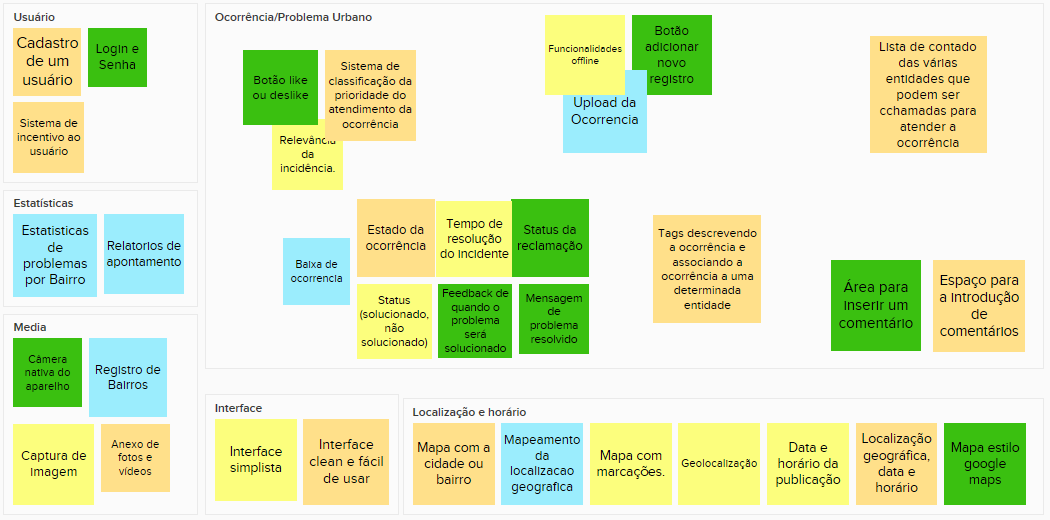
\includegraphics[scale=0.68]{cardsorting}
\caption{\textit{Card sorting} feito em sala de aula.}
\end{figure}

\clearpage

\section{Mapa de navegação e interação}
\begin{figure}[!ht]
\centering
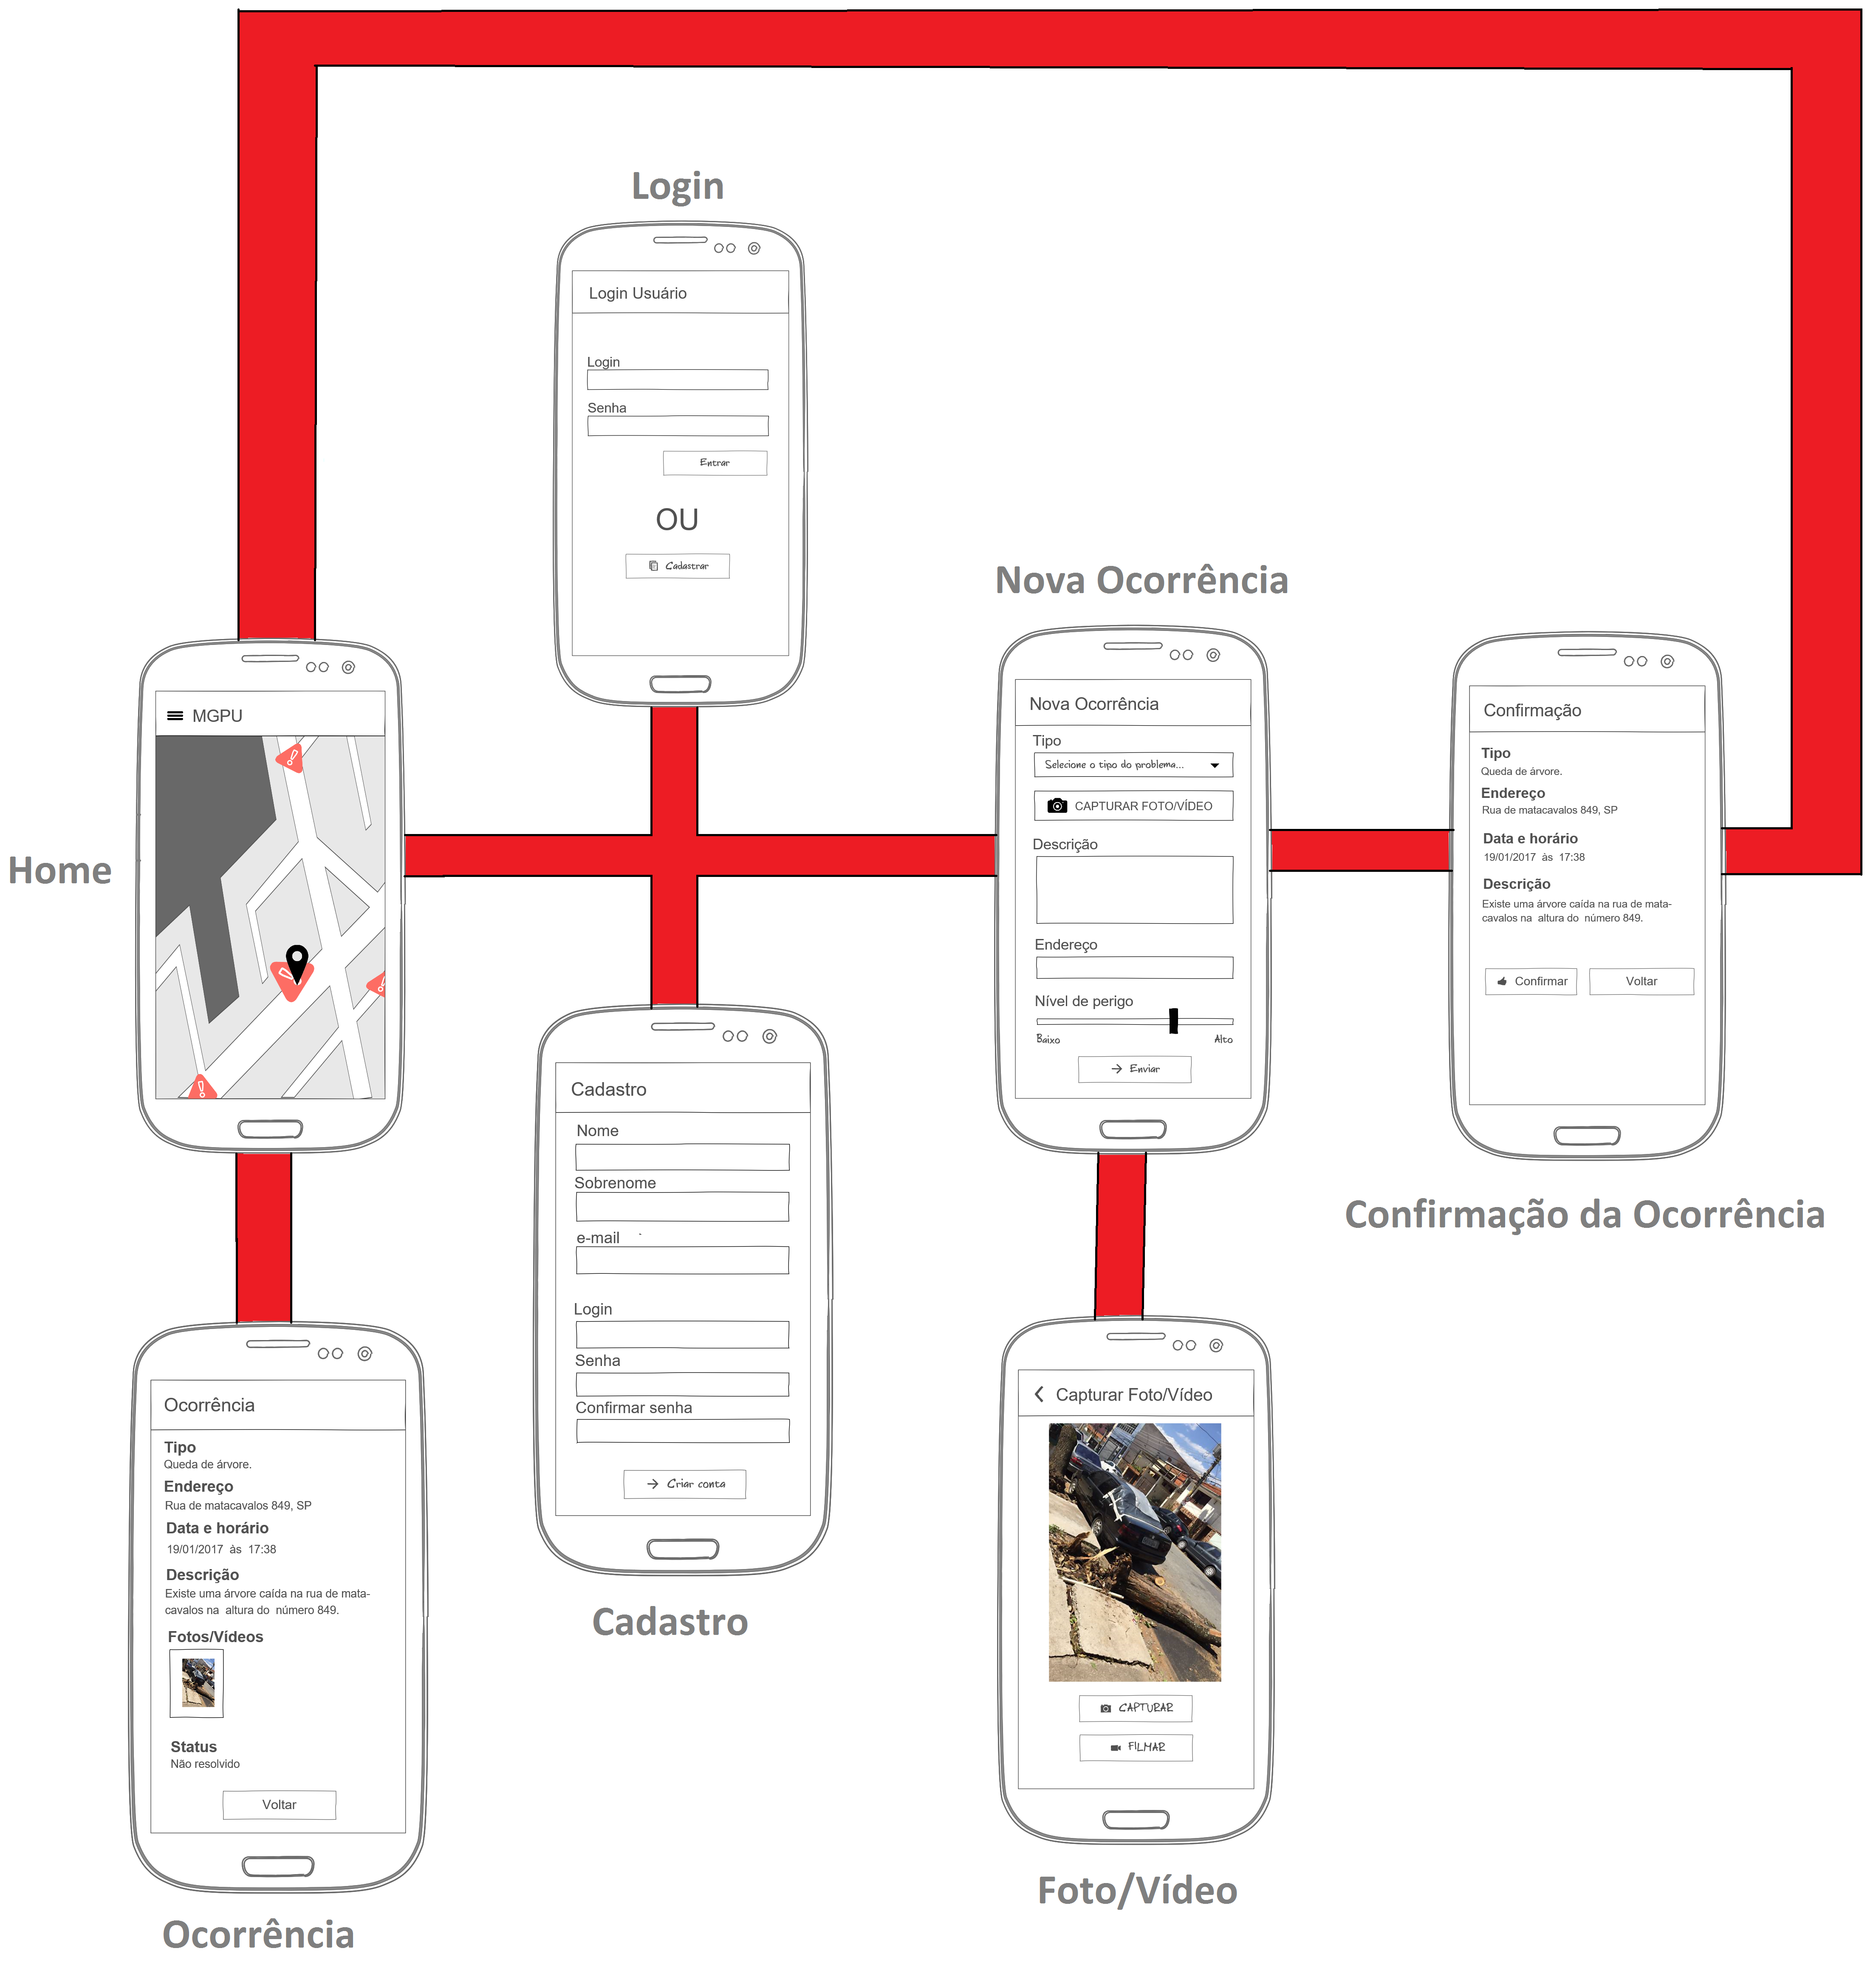
\includegraphics[scale=0.15]{mapaiter}
\caption{Mapa de navegação e interação simplificada do MGUP.}
\end{figure}

\chapter{Estudo de Cores}
De acordo com \cite{R0}, que mostra as características das cores, as associações atribuídas a cor verde, como de segurança, esperança, vegetação e natureza, foram as que que mais se relacionaram com a proposta do aplicativo (que é permitir aos cidadãos contribuir com a conservação, manutenção e segurança na cidade). Além disso, como dito em \cite{R0}, mais concretamente no arquivo Extra2 e página 36, o olho humano é mais sensível aos comprimentos de onda próximos ao amarelo-verde.
\\~\\
Foram utilizados conceitos do \textit{material design} que, de acordo com \cite{R3}, o principal objetivo é criar uma linguagem visual para os usuários que sintetize os princípios clássicos de um bom design com a inovação e as possibilidades da tecnologia e da ciência.
\\~\\
Também foram utilizado a paleta de cores Teal, que segundo \cite{R3} uma paleta de cores é composta por uma cor primária e outras cores de assentamento que foram projetadas para trabalhar de forma harmoniosa uma com as outras. A cor primária deve ser usada como cor principal do aplicativo, e as demais cores devem ser usadas para aplicar em outros componentes, a fim de atribuir um contraste mais dinâmico à tela.

\begin{figure}[!ht]
\centering
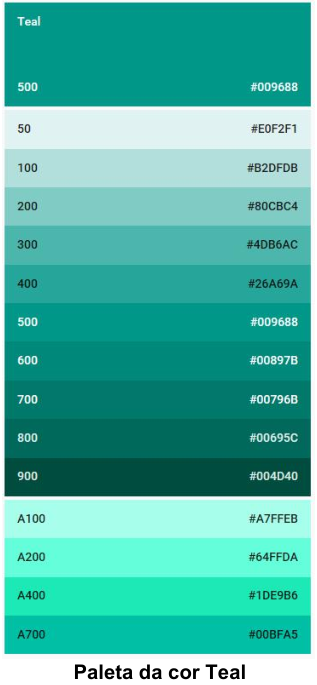
\includegraphics[scale=0.5]{teal}
\end{figure}
\ \\
Ainda é possível a utilização de uma paleta secundária para indicar um local relacionado a uma ação ou a uma informação que merece mais destaque. A paleta secundária deve ter uma variação mais escura ou mais clara que a cor primária escolhida.
\\~\\
Assim sendo, foi escolhido o amarelo (Amber), que de acordo com \cite{R0} é uma das cores mais sensíveis para o olho humano e consegue passar informações rapidamente para os olhos dos usuários. Isso é importante, visto que quanto rápido o usuário compreender uma funcionalidade, mais rápido ele conseguirá usar o sistema.

\begin{figure}[!ht]
\centering
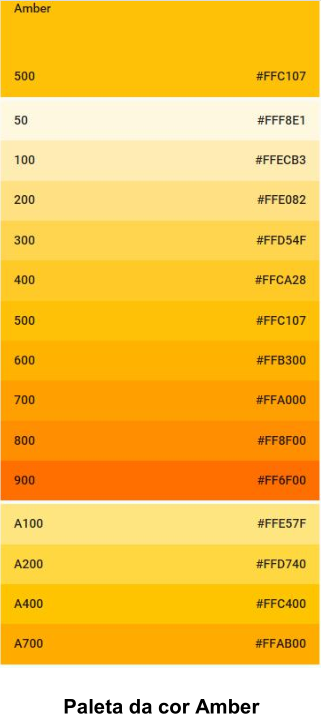
\includegraphics[scale=0.5]{amber}
\end{figure}
\ \\
A seguir temos uma imagem que ilustra o uso das cores primárias e secundárias que serão
utilizadas no projeto:

\begin{figure}[!ht]
\centering
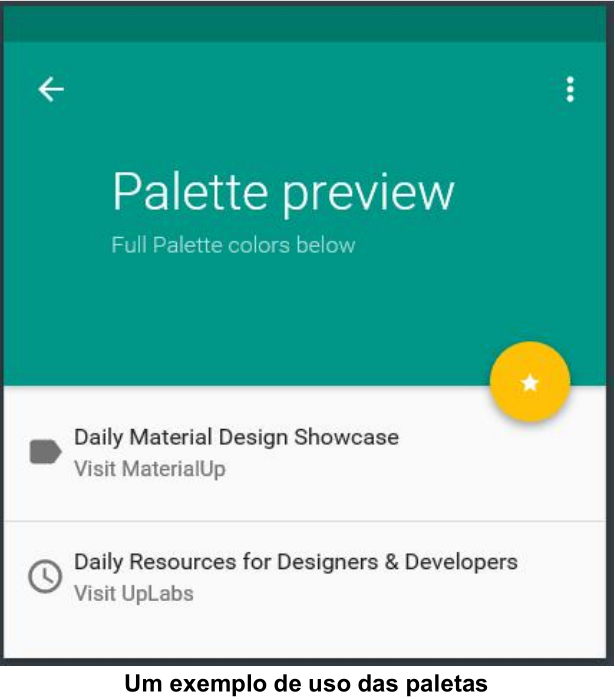
\includegraphics[scale=0.4]{exemplo}
\end{figure}

\chapter{Wireframes}
\textit{Wireframes} não são nada mais do que protótipos para a construção de telas de interação para aplicativos, páginas web, etc.\cite{R0} A construção desses protótipos deve-se ao fato de permitirem testar a viabilidade técnica da ideia, esclarecer requisitos vagos, realizar testes com usuário e auxiliam os \textit{designers} a optarem pelas melhores alternativas.\cite{R0}

\section{\textit{Wireframes} de baixa fidelidade}
\begin{figure}[!ht]
\centering
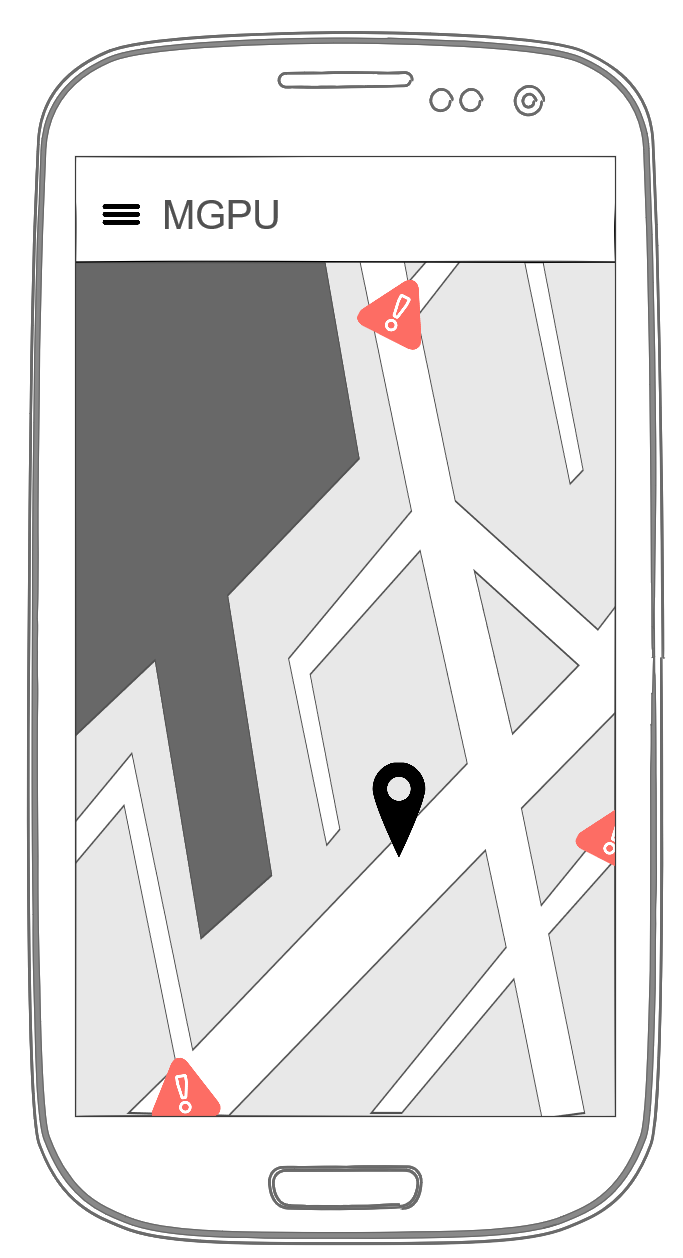
\includegraphics[scale=0.175]{wf1n}
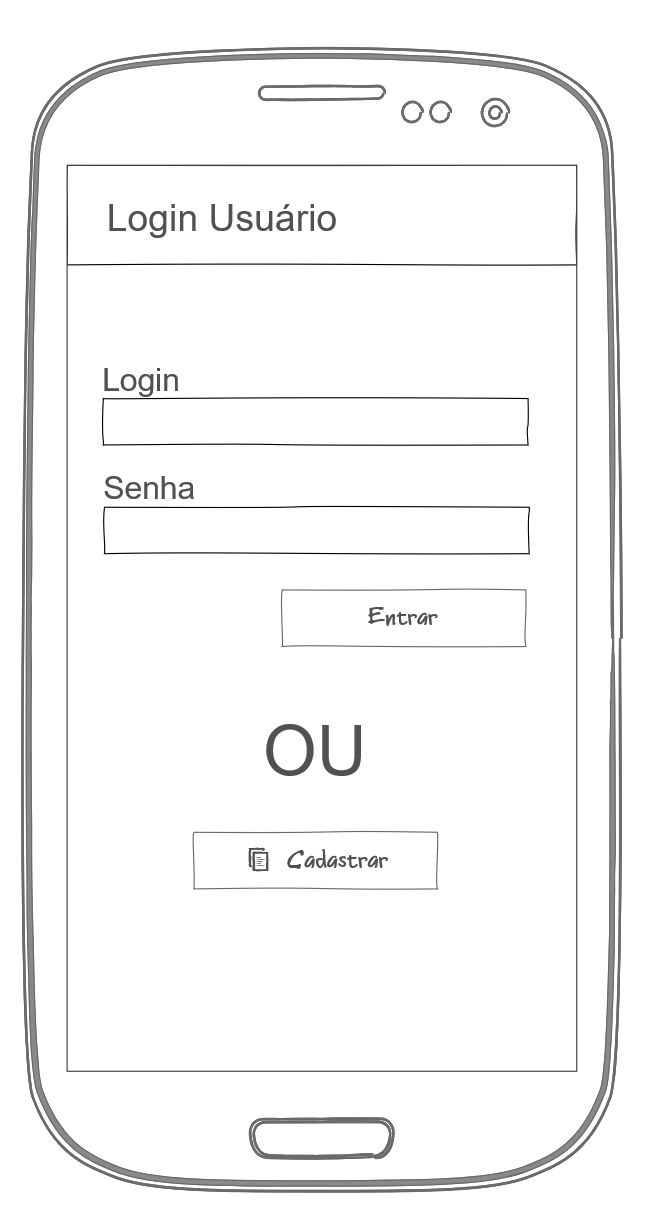
\includegraphics[scale=0.185]{wf2}
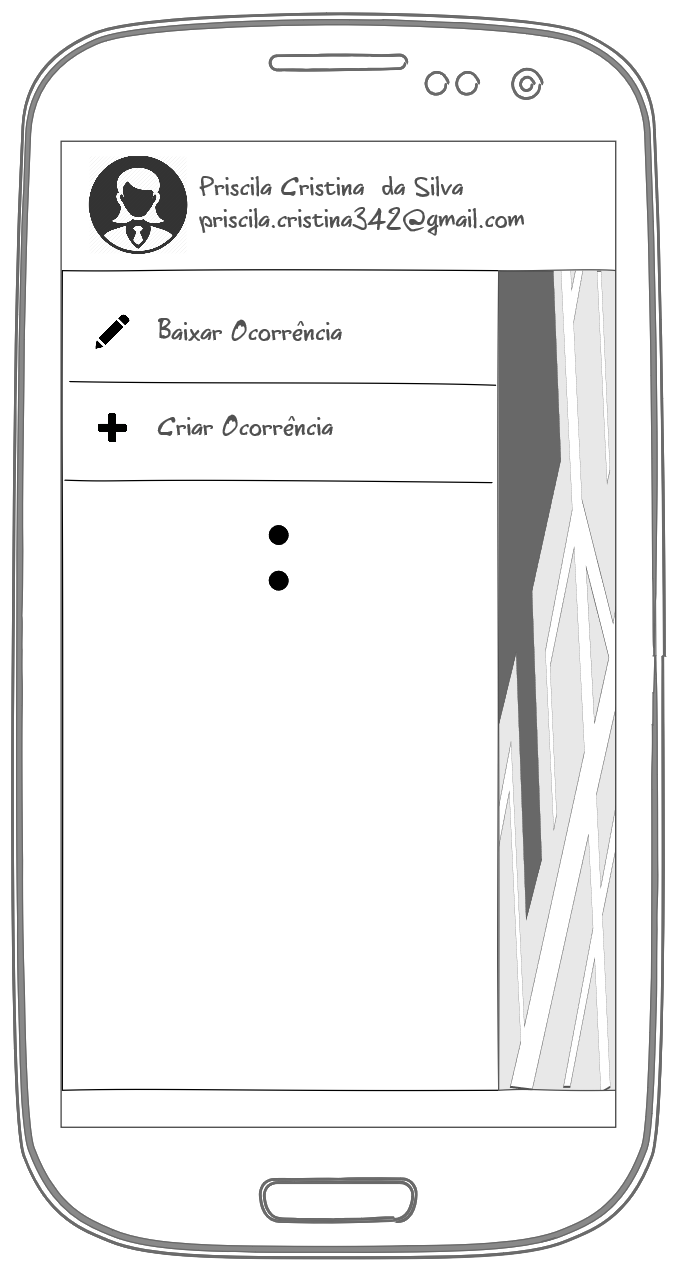
\includegraphics[scale=0.17]{wf3}
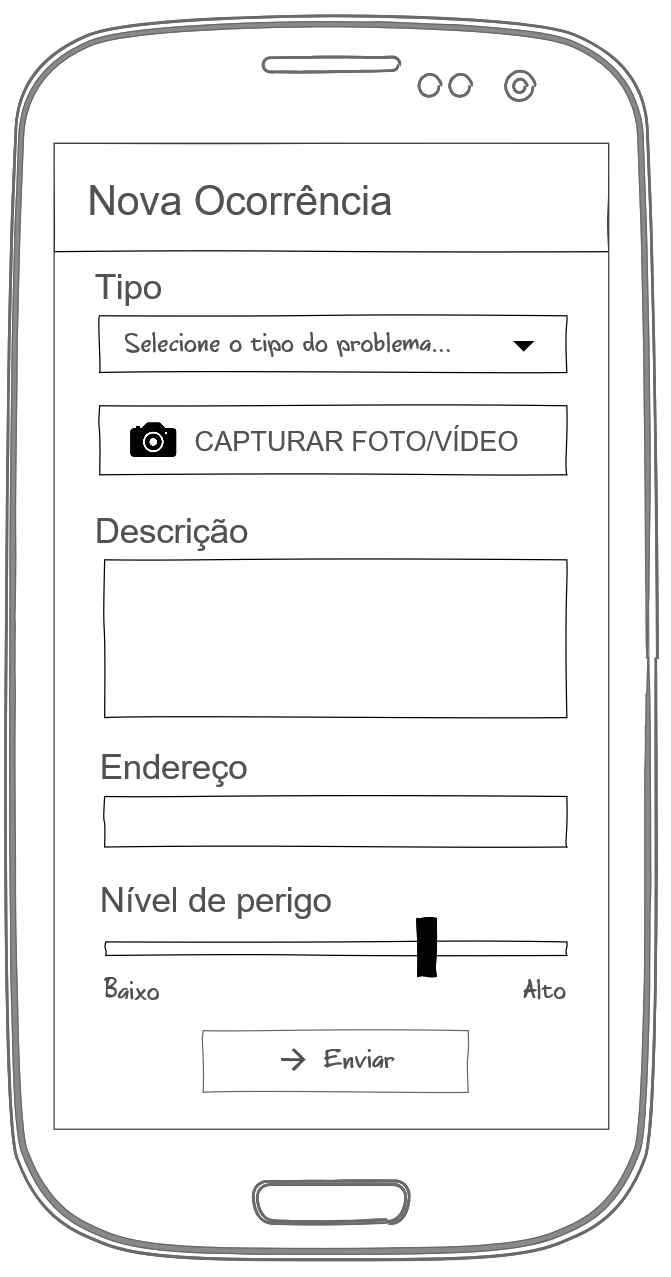
\includegraphics[scale=0.17]{wf4}
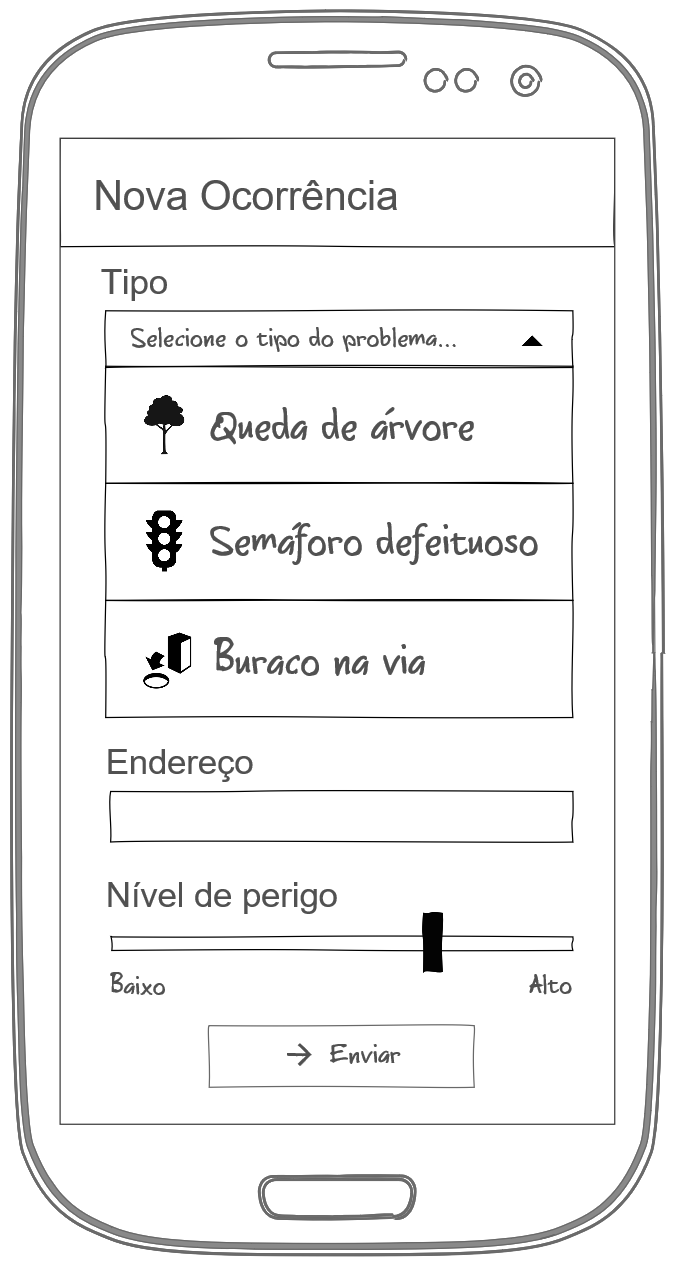
\includegraphics[scale=0.17]{wf5}
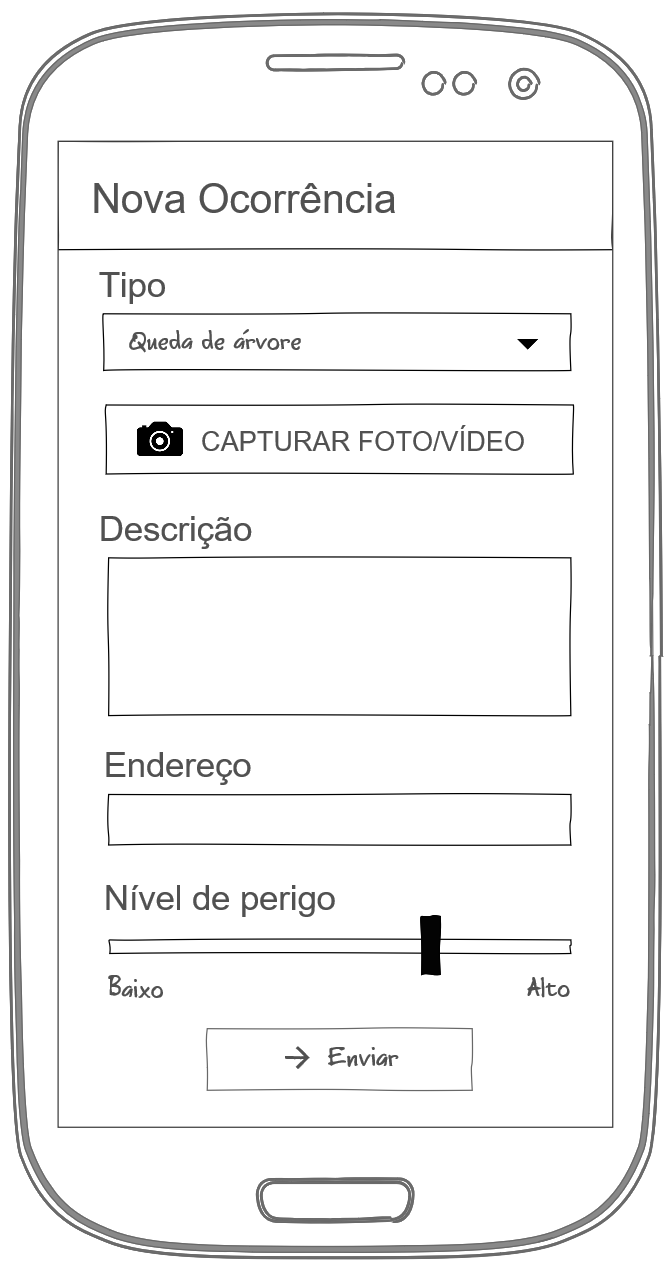
\includegraphics[scale=0.17]{wf6}
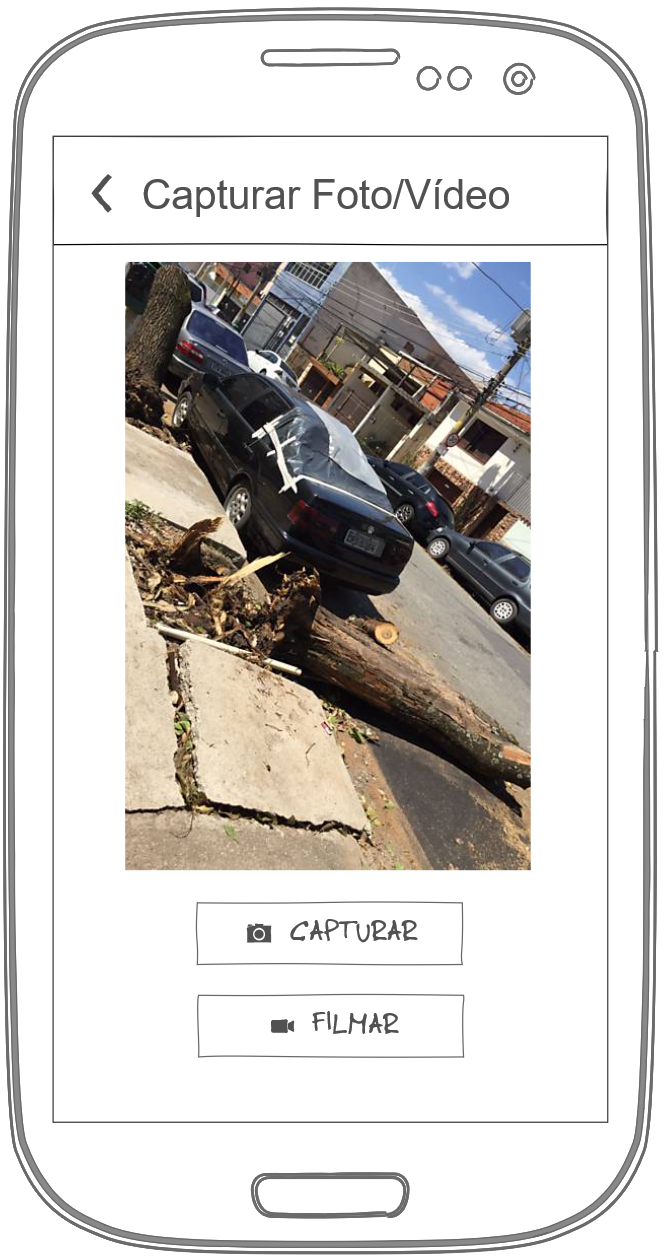
\includegraphics[scale=0.17]{wf7}
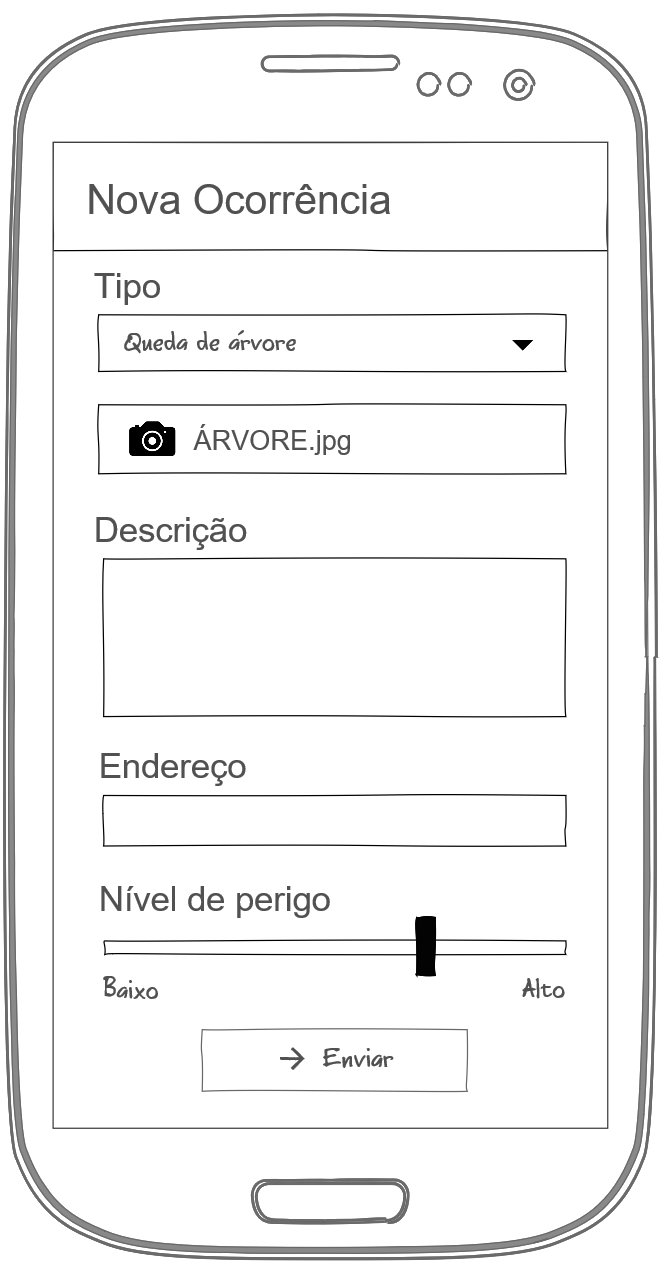
\includegraphics[scale=0.17]{wf8}
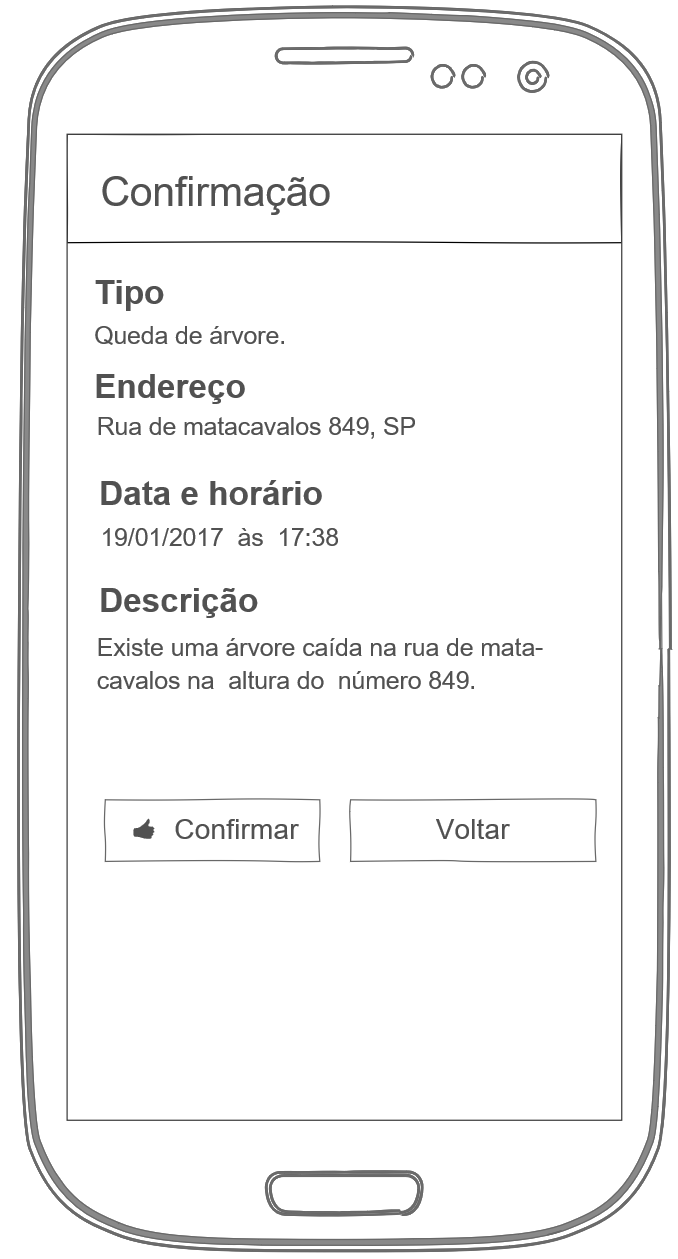
\includegraphics[scale=0.1715]{wf9}
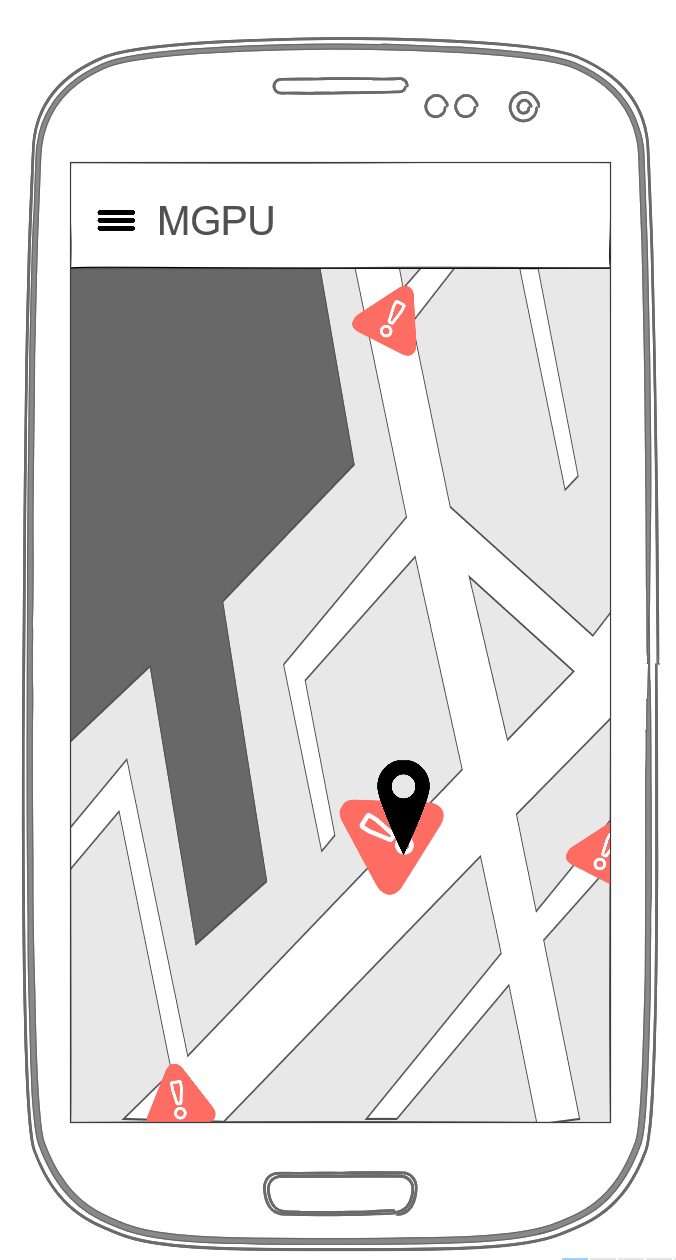
\includegraphics[scale=0.175]{wf10n}
\caption{\textit{Wireframe} de baixa fidelidade de um usuário reportando um problema urbano.}
\end{figure}

\clearpage

\section{\textit{Wireframes} de alta fidelidade}
\begin{figure}[!ht]
\centering
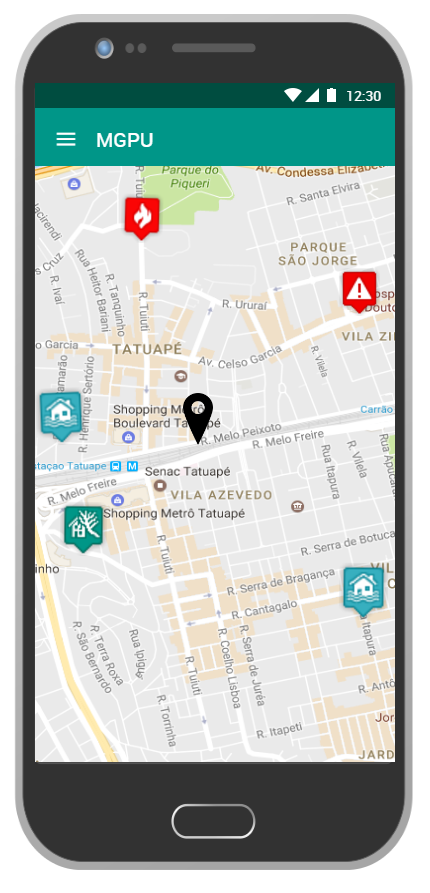
\includegraphics[scale=0.28]{twf1}
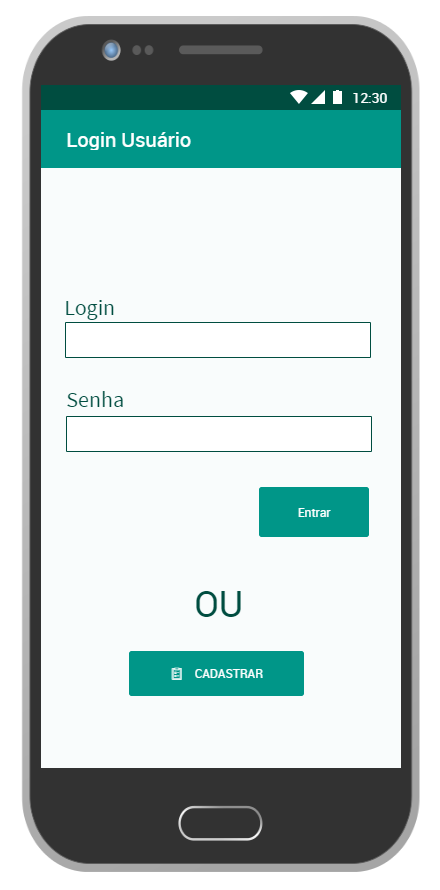
\includegraphics[scale=0.28]{twf2}
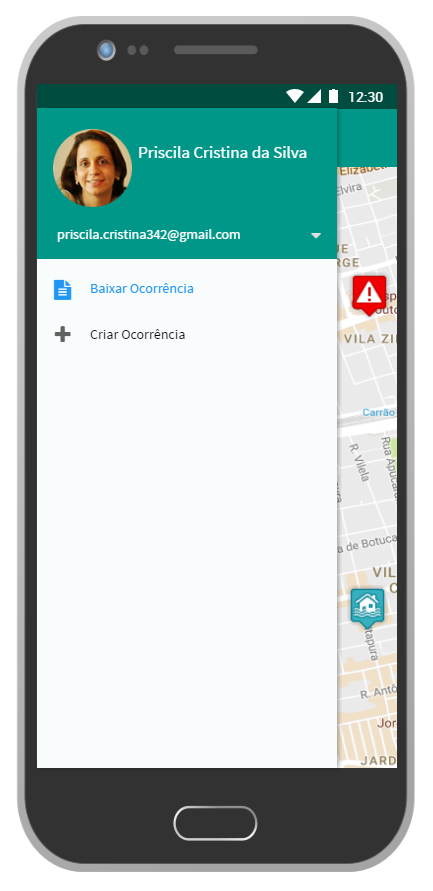
\includegraphics[scale=0.28]{twf3}
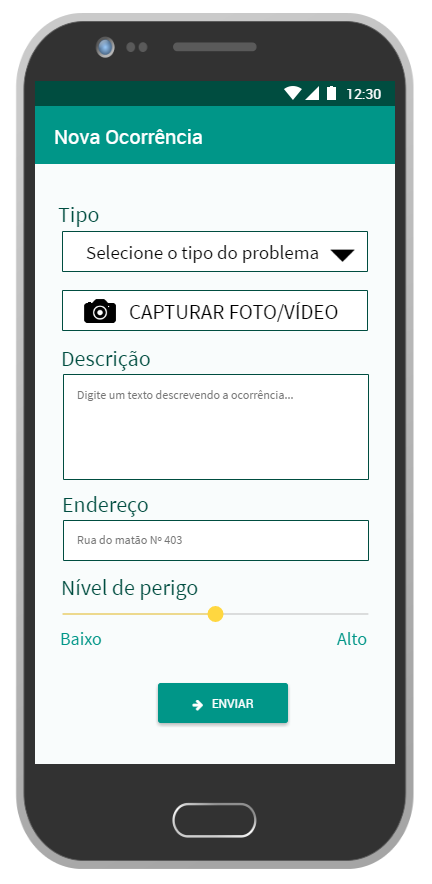
\includegraphics[scale=0.28]{twf4}
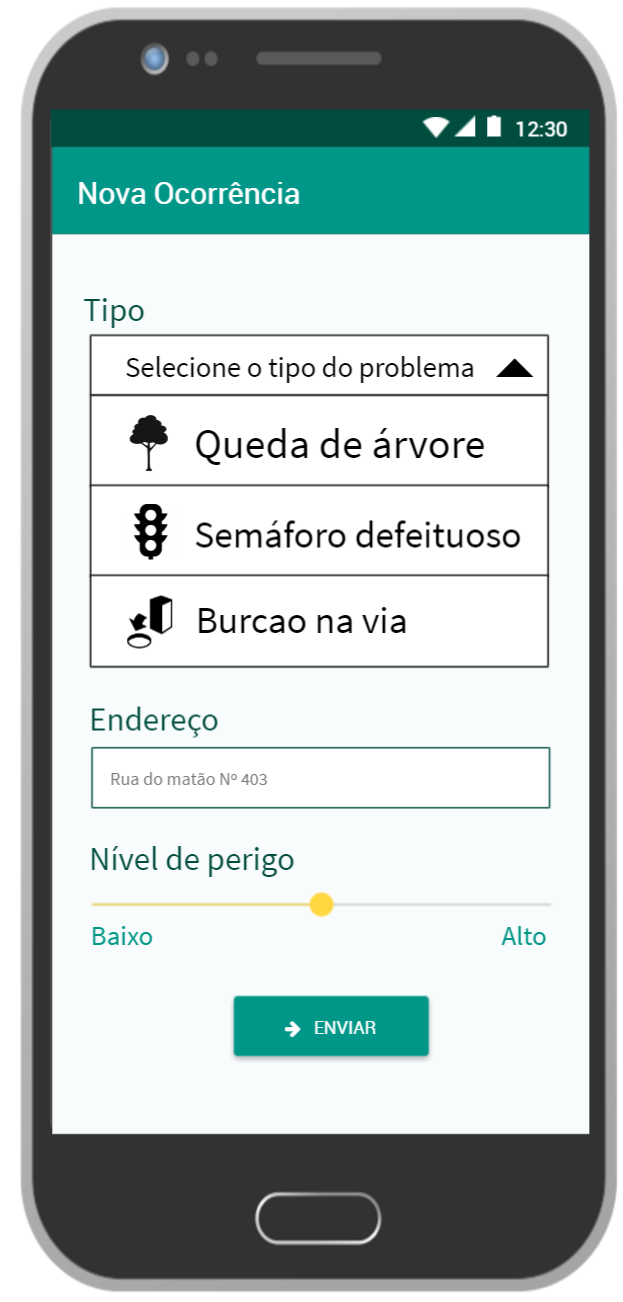
\includegraphics[scale=0.19]{twf5}
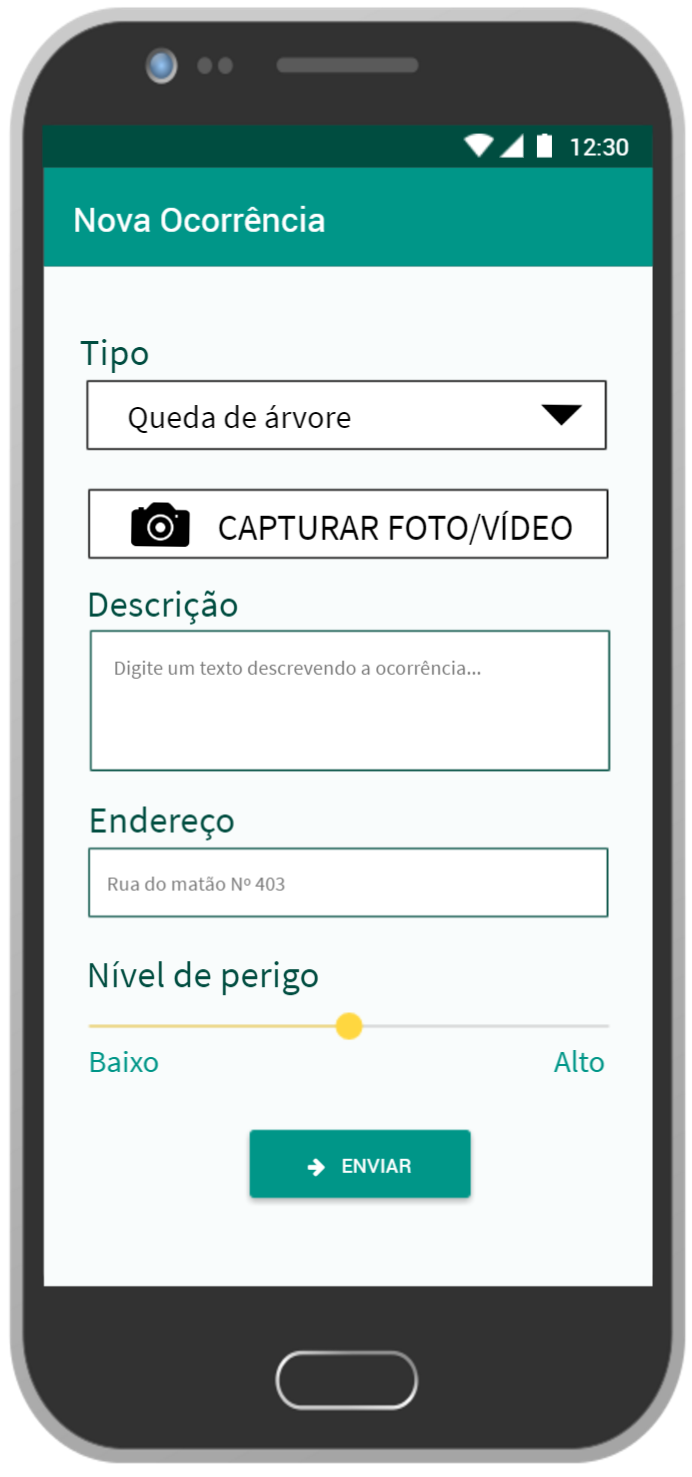
\includegraphics[scale=0.17]{twf6}
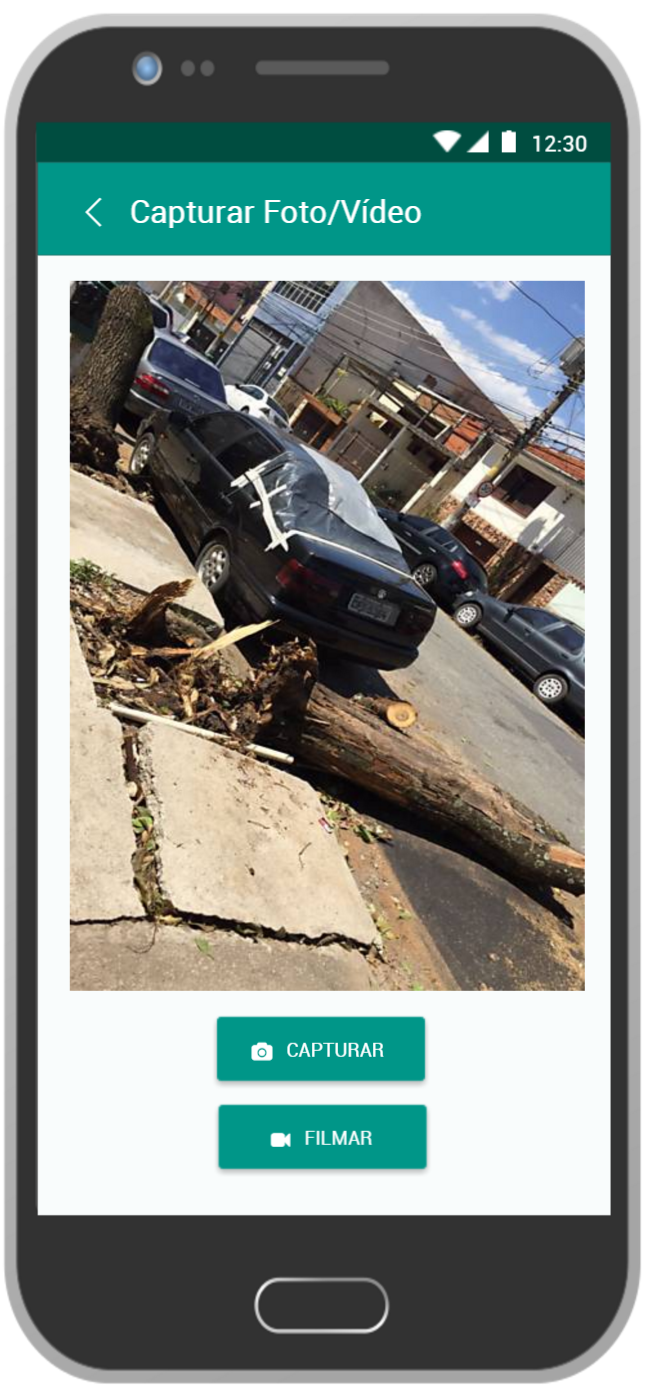
\includegraphics[scale=0.18]{twf7}
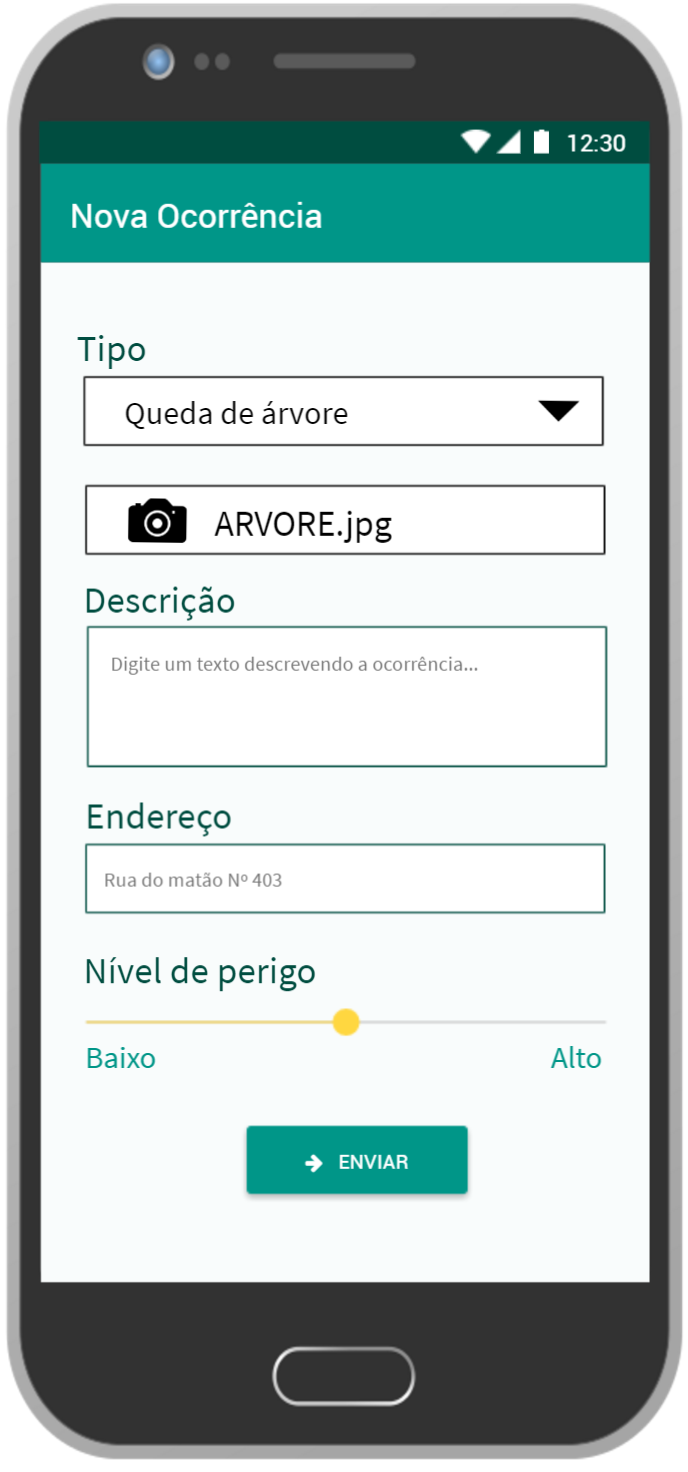
\includegraphics[scale=0.17]{twf8}
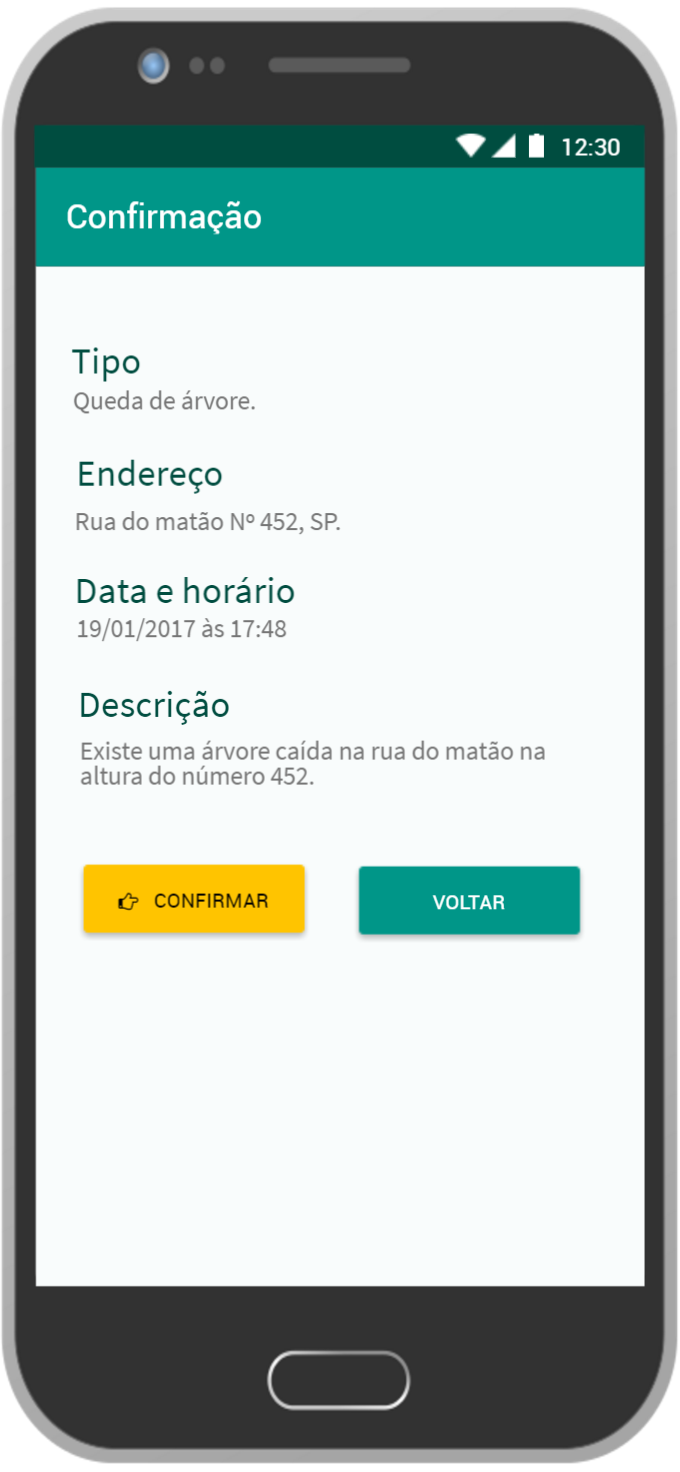
\includegraphics[scale=0.17]{twf9}
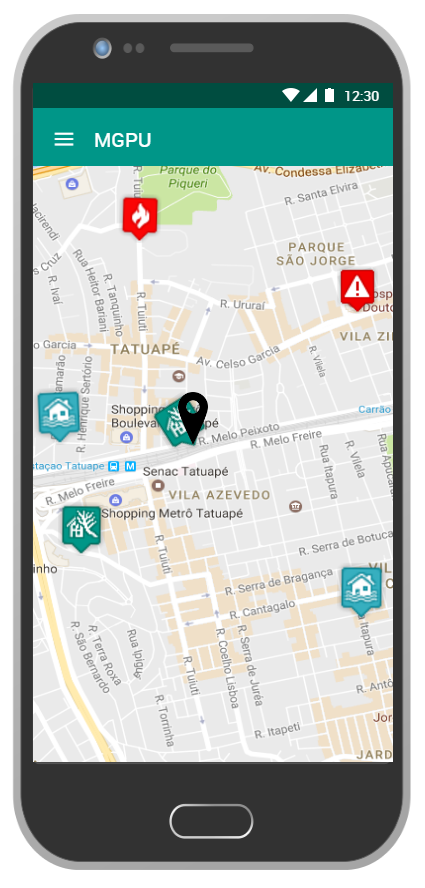
\includegraphics[scale=0.285]{twf10}
\caption{\textit{Wireframe} de alta fidelidade de um usuário reportando um problema urbano.}
\end{figure}


\chapter{UX Canvas}

Segundo \cite{R2}, o objetivo do \textit{UX Canvas} é oferecer ao designer uma ferramenta que o auxilie na concepção do projeto, na definição de objetivos, no entendimento do usuário e no desenvolvimento do produto, com base nas restrições apresentadas e nos recursos disponíveis.
\\~\\
Além disso o \textit{UX Canvas} permite ao designer manter o foco no conceito de experiência do uso do produto, ou seja, ao longo do desenvolvimento a experiência que se deseja oferecer ao usuário nunca é esquecida.\cite{R2}
\\~\\
Dito isso, eis o \textit{UX Canvas} que foi criado tendo em conta os requisitos do MGPU: 
\begin{figure}[!ht]
\centering
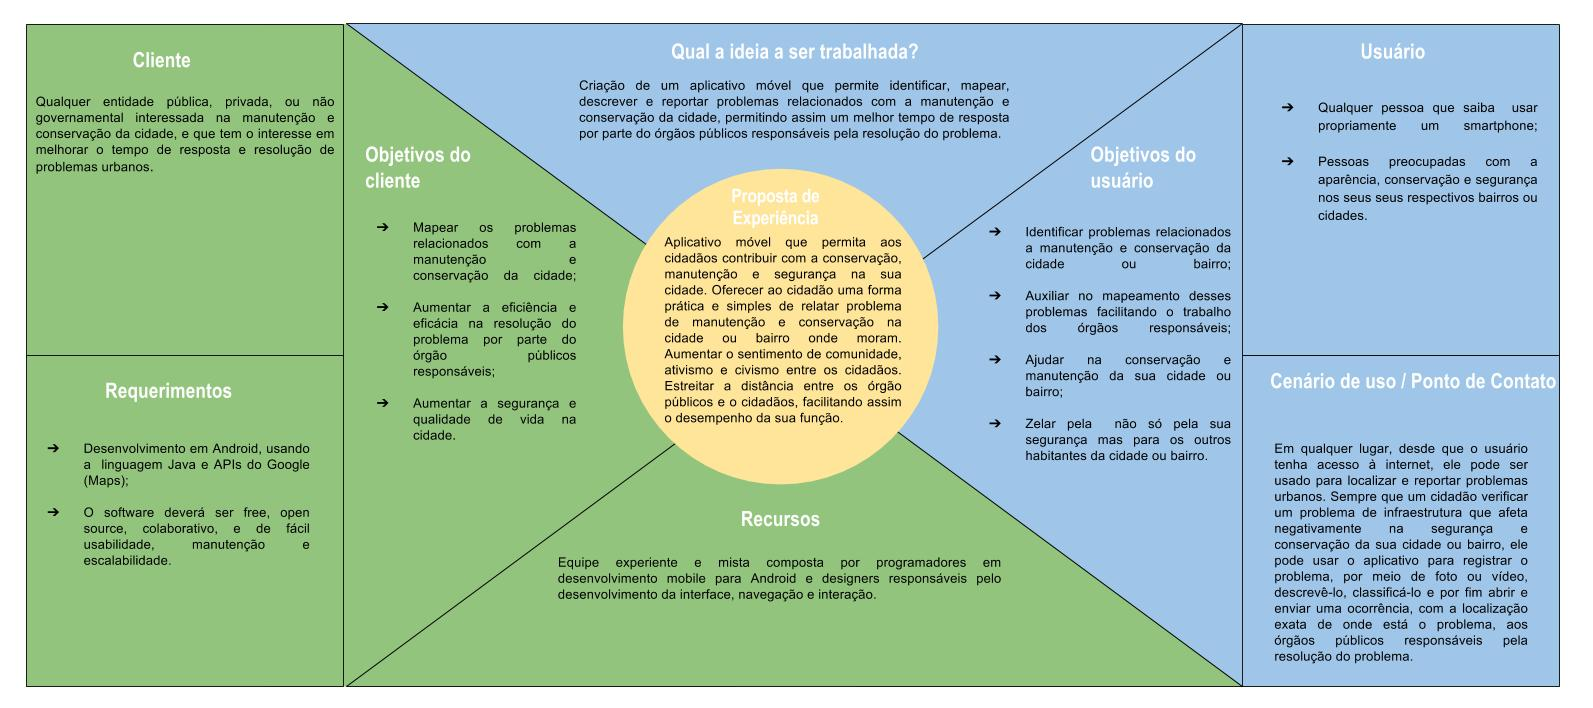
\includegraphics[scale=0.33]{uxcanvas}
\end{figure}

\chapter{Avaliação heurística}
A avaliação heurística consiste na verificação de uma interface por especialistas (normalmente entre 3 e 5), em relação a um conjunto reconhecido de regras, denominadas heurísticas de Nielsen (criador deste método de avaliação). Suas vantagens é que ela é uma avaliação de baixo custo e de fácil aplicação e identifica um grande número de pequenos problemas.\cite{R0}
\\~\\
Nas seções seguintes é feita uma avaliação heurística do aplicativo concorrente ao MGPU, o Cidadera\cite{R1}.

\section{Visibilidade do status do sistema}
\begin{itemize}
\item \textbf{Problema:} Os meios de \textit{feedback} ao usuário usados nesse aplicativo não são eficientes e eficazes.\\
  \textbf{Gravidade:} 1.\\
  \textbf{Solução:} Criar um mecanismo de \textit{push message} para alertar aos usuários sobre
novas ocorrências próximas deles.
\item \textbf{Problema:} O sistema poderia atualizar o mapa de tempos em tempos, visto que
  o botão para atualizar o mapa tem um contraste que não é de fácil visibilidade. Existe uma opção de ajuda
  que mostra as principais ações do
aplicativo, entretanto essa opção poderia estar mais visível.\\
\textbf{Gravidade:} 1.\\
\textbf{Solução:} Atualizar o mapa de tempo em tempos, colocar o botão para atualizar o
mapa num local de fácil acesso, e colocar o botão de ajuda fora
do menu lateral, visto que ele desaparece com frequência.
\end{itemize}

\section{Correlação entre o sistema e o mundo}
\begin{itemize}
\item \textbf{Problema:} O botão para abrir uma nova ocorrência é quase imperceptível, um novo
  usuário gastaria um tempo para descobrir como iniciar uma nova ocorrência.\\
\textbf{Gravidade:} 3.\\
\textbf{Solução:} Permitir que o usuário possa iniciar uma ocorrência dando dois toques no mapa,
ou então, um botão que deixasse explícito a ação de criar uma nova ocorrência.
\end{itemize}

\section{Controle e liberdade do usuário}
\begin{itemize}
\item O sistema permite que o usuário saia de situações e estados indesejados. 
\end{itemize}
    
\section{Consistência e padrões}
\begin{itemize}
\item A maioria das telas do aplicativo segue um padrão de cores preto e branco. No
  entanto, algumas telas fazem uso excessivo de várias cores diferentes, e isso pode atrapalhar
  a absorção de informações por parte dos usuários.\\
  \item \textbf{Problema:} Quando o usuário toca em uma marcação no mapa, surge uma janela mostrando
  as informações da ocorrência, o problema é que as cores
  escolhidas podem confudir o usuário, por exemplo, o botão para indicar que a
  ocorrência não foi resolvida tem fundo vermelho com uma fonte de cor branca,
  entretanto, o botão para indicar que o problema foi resolvido está com o fundo
  transparente e a cor da fonte é verde, dessa forma fica díficil notar o botão de
  resolvido em relação ao de não resolvido, e para piorar a situação, ambos estão muito próximos um do
  outro.\\
\textbf{Gravidade:} 2.\\
\textbf{Solução:} Alterar os estilos dos botões para que eles possam ser diferenciados
  pelos usuários.
\end{itemize}

\section{Prevenção de erros}
\begin{itemize}
  \item No geral o sistema prevê a maioria dos erros.
  \item \textbf{Problema:} O sistema não permite criar uma ocorrência \textbf{offline}. Assim um
  usuário que não tenha plano de internet móvel não poderá alertar ocorrências.\\
  \textbf{Gravidade:} 4.\\
  \textbf{Solução:} Criar um mecanismo que permita a criação de ocorrências mesmo que o
  usuário não tenha acesso à internet.
\item \textbf{Problema:} No caso de perda da conexão com a internet, o aplicativo trava durante a
  tentativa de visualizar uma marcação.\\
  \textbf{Problema:} 4.\\
  \textbf{Solução:} Manter em memória as informações referentes às
  ocorrências previamente carregadas no mapa, isso evitaria o problema.
\end{itemize}

\section{Reconhecimento ao invés de memorização}
\begin{itemize}
\item \textbf{Problema:} As principais funcionalidades do aplicativo não são de fácil reconhecimento
  , como por exemplo, iniciar uma nova ocorrência.\\
  \textbf{Gravidade:} 3.\\
  \textbf{Solução:} Permitir que usuário possa iniciar uma ocorrência dando dois cliques no
  mapa, ou então, ter um botão que deixasse explícito a ação de criar uma nova
  ocorrência.
\end{itemize}

\section{Flexibilidade e eficiência de uso}
\begin{itemize}
\item \textbf{Problema:} O aplicativo não permite que o usuário programe ou personalize suas
  ações frequentes.\\
  \textbf{Gravidade:} 1.\\
  \textbf{Solução:} Poderia ter uma tela de configurações, na qual o usuário poderia selecionar
  as ocorrências que ele mais costuma reportar, assim como as descrições que ele
  escreve e os tipos de problemas que ele seleciona.
\end{itemize}

\section{Projeto estético e minimalista}
\begin{itemize}
\item \textbf{Problema:} A aparência do aplicativo relembra os aplicativos desenvolvidos no ano 2010, a cor utilizada passa uma sensação de tristeza.\\
  \textbf{Gravidade:} 3.\\
  \textbf{Solução:} Utilizar os conceitos do \textit{material design}\cite{R3} para escolher
  esquemas de cores que se relacionam entre si. Escolher cores que passam uma
  sensação de segurança e comodidade.
\end{itemize}

\section{Suporte aos usuários no reconhecimento, diagnóstico e recuperação de erros}
\begin{itemize}
\item No geral e quando necessário, o aplicativo informa ao usuário quando uma
  funcionalidade não pode ser usada devido à falta de conexão à internet.
\item \textbf{Problema:} O aplicativo fecha quando o usuário tenta abrir uma marcação
  mas não existe conexão com a internet. Ao abrir o aplicativo
  nenhuma mensagem informado o motivo do erro é apresentada. Assim o
  usuário não tem como evitar o erro.\\
\textbf{Gravidade:} 4.\\
\textbf{Solução:} Apresentar uma mensagem informando o que ocasionou o erro.
\end{itemize}

\section{Informações de ajuda e documentação}
\begin{itemize}
\item O sistema possui uma opção de ajuda que mostra aos usuários qual é a função de
cada botão na interface do aplicativo.
\end{itemize}

\chapter{Roteiro de teste de usabilidade}

Para a realização dos testes de usabilidade é necessário ter bem definido os objetivos, as métricas, os participantes, as tarefas e os cenários, visto que os resultados desses testes, quando bem feitos, facilitam na validação fluxos, layouts e funcionalidades.\cite{R0,R4}

\section{Objetivos}
\begin{itemize}
\item Compreender a função principal do aplicativo – Encontrar e registrar ocorrências relacionadas a problemas urbanos.
\begin{itemize}
\item O usuário compreende a necessidade de se registrar no sistema e realizar o registro e acompanhamento da ocorrência?
\item O usuário possui uma dificuldade em realizar o registro da ocorrência?
\item O usuário assimila as etapas de navegação e visualização do mapa com suas respectivas ocorrência?
\item O usuário consegue passar por todas as etapas chegando ao objetivo final de forma intuitiva?
\end{itemize}
\item O usuário interage de forma clara com a visualização dos itens de uma ocorrência.
\begin{itemize}
\item Na tela de exibição do mapa, o usuário considera que essa seja uma forma útil e prática de registrar uma ocorrência?
\item Na tela de registro de ocorrência a navegação é mostrada de forma que facilita a usabilidade por parte do usuário?
\item As informações proposta no mapa são mostradas de forma que permita a identificação rápida e eficiente da ocorrência?
\end{itemize}
\item O usuário recebe \textit{feedbacks} eficazes.
\begin{itemize}
\item O aplicativo fornece instruções e informações, claras ou subentendidas, sobre os passos que deve seguir para registrar uma ocorrência?
\item O aplicativo indica de forma clara as mudanças de estado para se chegar ao objetivo final do mesmo?
\item O aplicativo informa sobre seu funcionamento para que o usuário saiba qual o próximo passo a ser executado de forma a consolidar o registro da respectiva ocorrência?
\end{itemize}
\end{itemize}

\section{Métricas}
\begin{itemize}
\item Erros que o usuário pode cometer ao realizar uma ocorrência;
\begin{itemize}
\item Verificar o tempo que o usuário leva para se registrar no sistema no momento da primeira ocorrência;
\item Verificar se o usuário pode atualizar os dados já fornecidos;
\item Identificar se o usuário percebe claramente as entradas e saídas do produto;
\item Existência de um sistema de ajuda no aplicativo.
\end{itemize}
\item Satisfação.
\begin{itemize}
\item Mensurar o grau de atendimento as necessidades do usuário, ao nível de conteúdo da informação;
\item Avaliar o tempo que o usuário novato leva para aprender a usar o aplicativo;
\item Verificar o número de comandos, menus, ou ícones que o usuário deve conhecer ou acessar para obter a informação desejada é satisfatório.
\end{itemize}
\end{itemize}

\section{Perfil dos participantes}
\begin{itemize}
\item \textbf{Carla Patrícia Cavalcanti:} Carla tem 40 anos, casada e mãe de dois filhos. Ela é muito devota aos filhos e na medida do possível tenta dar tudo do melhor para eles. Trabalha como recepcionista num escritório na Avenida Paulista e usa como principal meio de transporte o metrô. 
\item \textbf{Marcos Almeida:} Marcos faz bacharelato em letras, é uma pessoa muito atenciosa e compreensiva, adora viajar e conhecer pessoas novas. Na faculdade ele faz parte da comissão de recepção dos calouros do curso de letras.
\item \textbf{Luís Carlos:} Doutorado em Psicologia, Luís é professor universitário e coordenador do curso de psicologia. Passa maior parte do tempo fazendo pesquisas, é separado e tem um filho já adulto. Apesar de ser uma pessoa muito ocupada, ele está sempre disposto a ajudar.
\end{itemize}
\section{Tarefas e cenários}
\subsection{Tarefas}
\begin{itemize}
\item Fazer o registro no aplicativo e realizar uma nova ocorrência anexando um vídeo como prova de autenticidade da mesma.
\item Realizar uma nova ocorrência, selecionar o tipo da ocorrência, registrar uma foto do cenário, escrever uma descrição da ocorrência, identificar o endereço da ocorrência e o seu nível de perigo.
\item Abrir uma ocorrência no mapa e verificar o tipo da ocorrência, a perigosidade e o seu \textit{status} atual.
\end{itemize}
\subsection{Cenários}
\begin{itemize}
\item Muitas vezes, para desviar de buracos, motoristas invadem a pista contrária. "Parece que o asfalto não suporta nem um dia de reparos". O problema maior é na segurança dos pedestres, estes correm o risco de serem ofuscados por um farol, o que reduz a visibilidade e o tempo de reação de uma pessoa, e por conseguinte a probabilidade de acidentes fatais aumenta. 
\item A Zona Oeste da capital paulista apresenta árvores caídas por suas vias nesta segunda-feira, quatro dias após o temporal que atingiu a cidade. As chuvas das tardes também causaram falta de energia elétrica em diversos pontos da cidade, especialmente na região oeste. Como poderíamos detectar e registra tais quedas de arvores na cidade?
\item Calçadas esburacadas têm preocupado e colocado em risco a vida dos moradores da cidade de São Paulo. Além dos buracos, os pedestres reclamam da falta de sinalização alertando para o risco de acidentes.
\end{itemize}

\chapter{Conclusão}

Infelizmente, dado que o curso é de curta duração, não foi possivel prototipar todas as funcionalidades que foram levantadas e exploradas durante o \textit{card sorting}, mas as poucas funcionalidades prototipadas foram suficientes para praticar a maioria dos conceitos e técnicas vistas ao longo do curso, usar as diversar ferramentas colaborativas de \textit{design} e prototipação apresentadas pelo professor, e por fim realizar que a construção de qualquer produto, tendo em conta a maximização da usabilidade e experiência do usuário, é uma tarefa complexa, muito exigente e com custos que podem ser elevados.
\\~\\
O curso e o trabalho final foram de uma importância tremenda, todos os membros da equipe notaram uma evolução positiva no que diz respeito ao domínio dos principais conceitos de engenharia de usabilidade.

\begin{thebibliography}{9}

\bibitem{R0}
JUNIOR, Hamilton Fernandes de Moraes. Engenharia de usabilidade. 16-20 de jan de 2017. Materiais da aula. 

\bibitem{R1} 
{\it Cidadera}. Disponível em: \textless http://cidadera.com/ \textgreater. Acesso em: Janeiro 2017.

\bibitem{R2} 
{\it UXCanvas}. Disponível em: \textless http://uxcanvas.com/ \textgreater. Acesso em: Janeiro 2017.

\bibitem{R3} 
{\it Material Design}. Disponível em: \textless https://material.io/guidelines/material-design/introduction.html \textgreater. Acesso em: Janeiro 2017.

\bibitem{R4} 
TEIXEIRA, Fabricio. Introdução e boas práticas em UX Design. São Paulo: Casa do Código, 2015. 271.

\bibitem{R5} 
AHITUY, N. Principles of information system for management. 3nd.ed. Dubuque, EUA: WCB, 1990. 653 p.

\bibitem{R6} 
FREITAS, Henrique M. R. et al. Avaliação de sistemas de informações. Revista de Administração, São Paulo, v. 29, n.4, p 36-55, out/dez 1994.

\bibitem{R7} 
JACSÓ, P. CD-ROM software, dataware and hardware: evaluation, selection, and installation. Englewood, CO: Libraries Unlimited, 1992.


\end{thebibliography}

\vfill
\end{document}
